\section{Results}

To simulate the inhibition of HDAC6-mediated uncoating by DARPin-F10 we created two new HDAC6 complex formation models: "Symmetric DARPin" and "Asymmetric DARPin" (Figure \ref{figure:darpinReactionModelSchemes}, see Appendix \ref{appendix:DARPinModelsEquations} for details) based respectively on "Symmetric" and "Asymmetric" model variants, as reported in Chapter \ref{ch:ReactionModels}. The key difference between them follows from the structure of the original models. Ub only assists the binding of myosin in the "Asymmetric" model, so the presence of DARPin-F10 would only inhibit myosin recruitment, while for the "Symmetric" model DARPin-F10 would affect the recruitment of both myosin and dynein motors.

\begin{figure}
\begin{center}
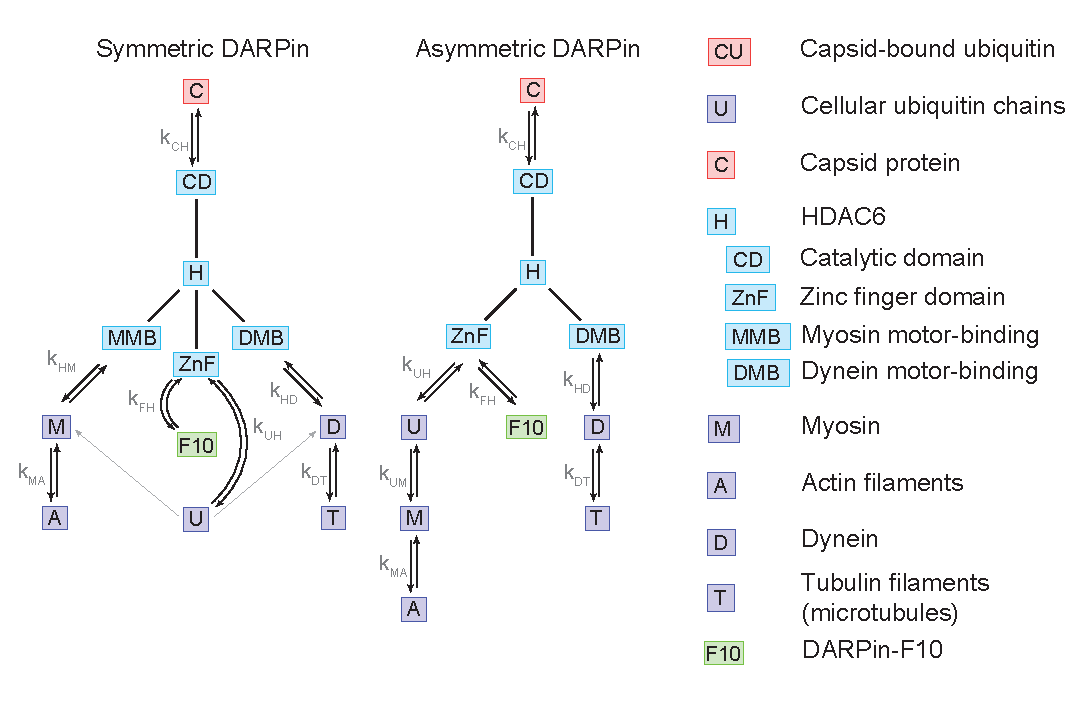
\includegraphics[width=0.95\textwidth, trim={0cm 0cm 0cm 0cm}, clip]{D_chapters/3_DARPinModels/ReactionModelSchemesDarpin.pdf}
\caption[HDAC6 complex formation models densities with and without DARPin-F10]%
{Interaction schematics for the two DARPin-F10 reaction model variants. Nodes represent proteins or protein domains (linked by solid lines) and arrows denote biochemical reactions with corresponding on-rates indicated next to the arrows. Node colors distinguish between viral proteins (red), HDAC6 (cyan), other host proteins (purple), and DARPin-F10 (green).}
\label{figure:darpinReactionModelSchemes}
\end{center}
\end{figure}

\begin{figure}
\begin{center}
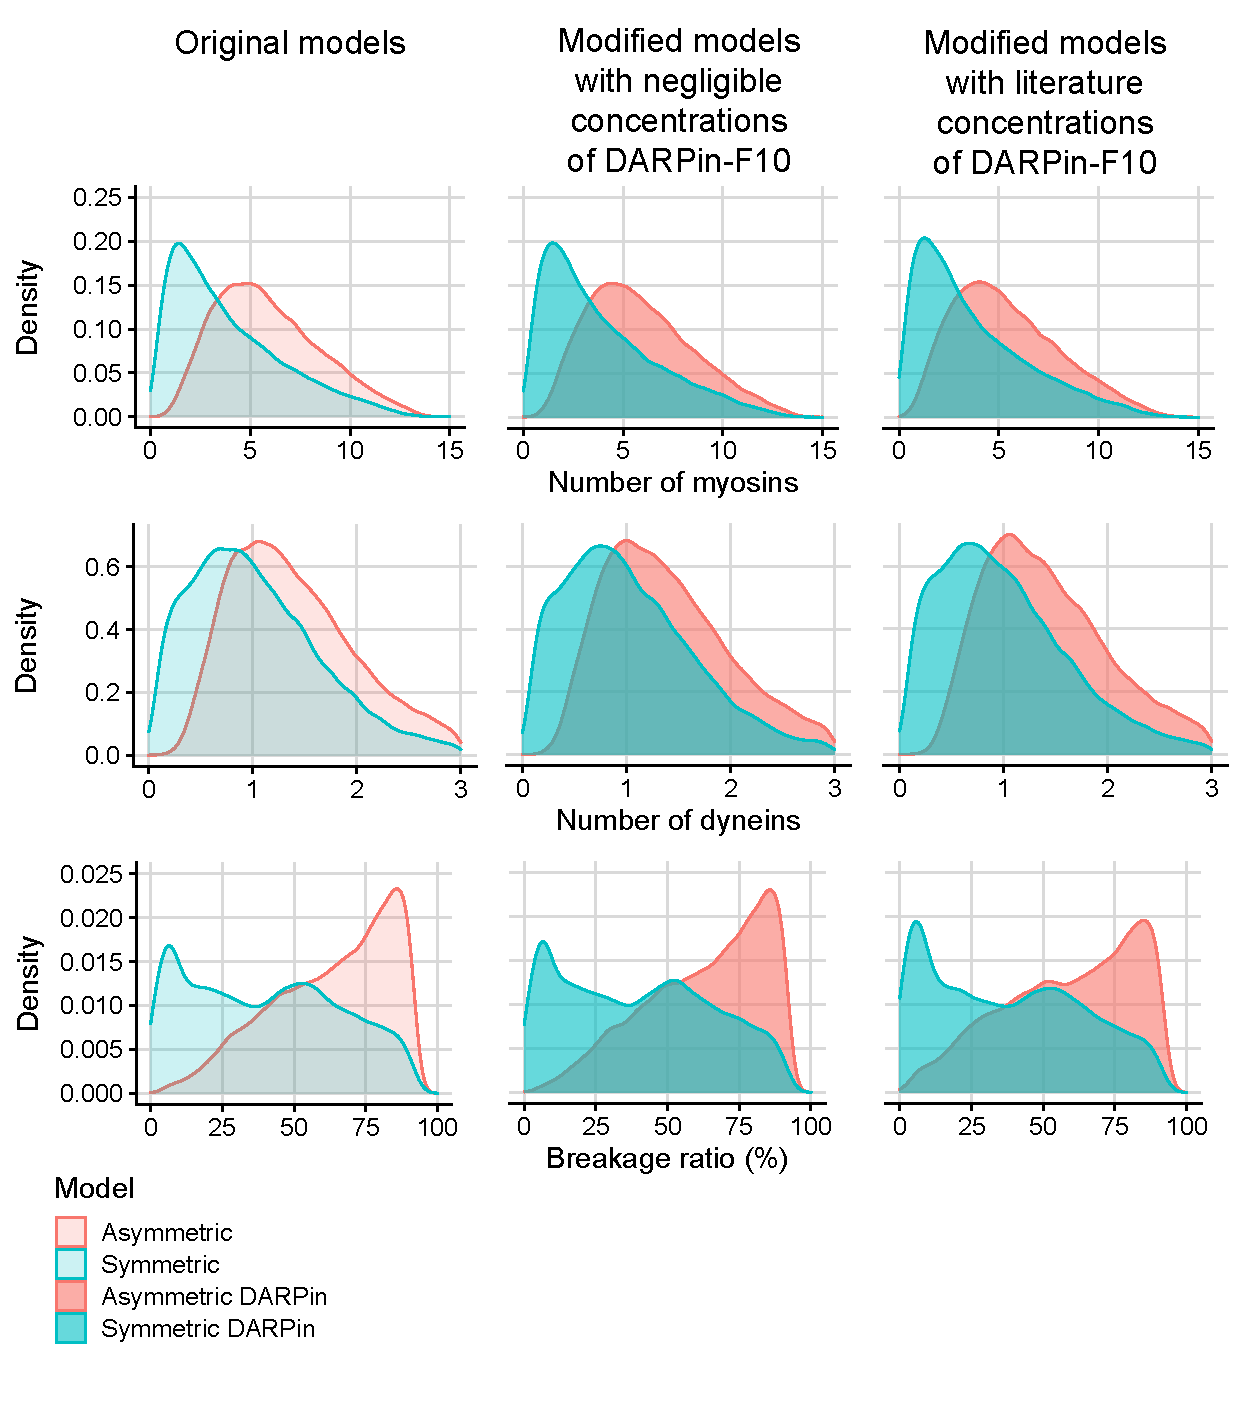
\includegraphics[width=0.95\textwidth, trim={0cm 0cm 0cm 0cm}, clip]{D_chapters/3_DARPinModels/Density_DARPin.pdf}
\caption[HDAC6 complex formation models densities with and without DARPin-F10]%
{HDAC6 complex formation models densities with and without DARPin-F10.\par
Arrows are aligned to highlight the change in the density between the original model and the modified DARPin-F10 model.}
\label{figure:darpinDensities}
\end{center}
\end{figure}

To verify that the base reaction network of our modified HDAC6 models functions as before, we uniformly sampled reactions and rates around our starting point for two concentrations of DARPin-F10 - one negligibly small, and $34.7$ nM - value compatible with DARPin concentrations previously reported in literature \cite{guillard2017structural} (Figure \ref{figure:darpinDensities}, see Methods \ref{ch:DARPinMethods} for detail). Modified models with negligible concentrations of DARPin-F10 performed largely the same as before. While the difference in densities for DARPin-F10 for literature reported concentrations is mild, it is clear that for the modified "Asymmetric DARPin" model the peak of myosin recruitment is shifted slightly from 5 to 4 compared to the original model. Likewise, the modified "Symmetric DARPin" model on average recruits slightly fewer dyneins than the original model. These changes in motor recruitment lead to a density increase in the low capsid breakage ratio for the "Symmetric DARPin" model and a density decrease of high capsid breakage ratio for the "Asymmetric DARPin" model (Figure \ref{figure:darpinDensities}).

\begin{figure}
\begin{center}
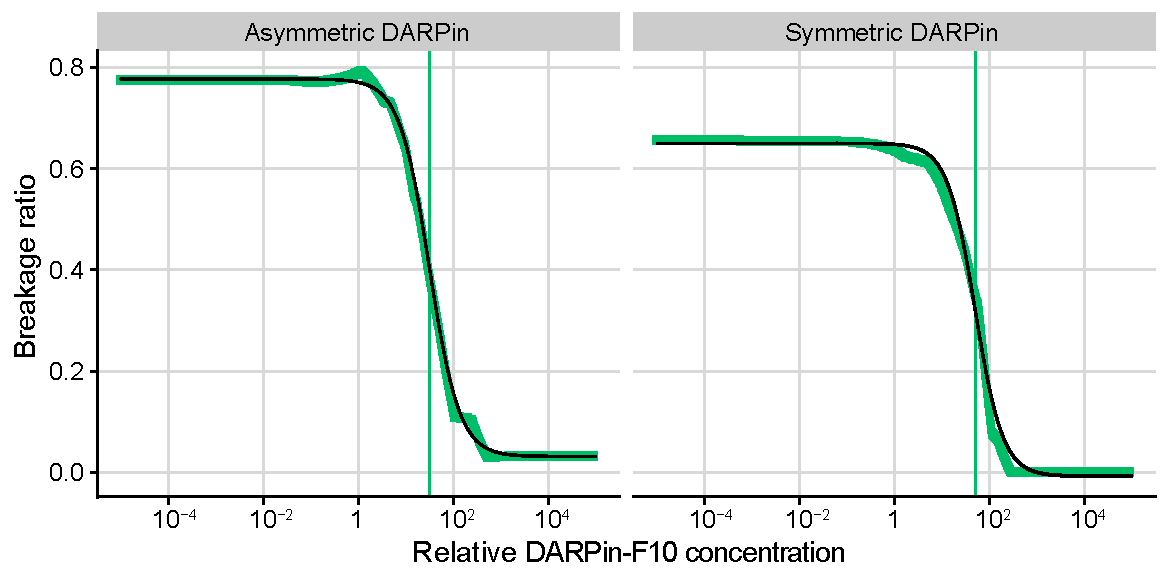
\includegraphics[width=0.95\textwidth, trim={0cm 0cm 0cm 0cm}, clip]{D_chapters/3_DARPinModels/FitDarpinTrajectories.pdf}
\caption[Capsid breakage prediction depending on relative DARPin-F10concentration]%
{Capsid breakage prediction depending on relative DARPin-F10 concentration. \par
The green trajectory is a direct prediction from the model, the black line is a corresponding Hill equation fit. All the concentrations are relative to literature value $34.7$ nM, corresponding to 1 on the plot. The vertical green line denotes EC50 value of the fit.}
\label{figure:darpinTrajectories}
\end{center}
\end{figure}

To simulate influenza uncoating dose response to DARPin-F10 we widely sampled the DARPin-F10 concentration near the literature value, and ran simulations for both "Symmetric DARPin" and "Asymmetric DARPin" models of HDAC6 complex formation. Both models displayed similar sigmoidal behavior for DARPin-F10 (Figure \ref{figure:darpinTrajectories}). At low concentrations the breakage ratio for both models stayed approximately the same as before (Figure \ref{figure:sampledTrajectories}), with the "Asymmetric DARPin" model variant achieving higher capsid breakage. Increasing DARPin-F10 concentration lead to a dramatic drop in the observed capsid breakage ratio.

To characterize resulting trajectories we fitted them using the Hill equation for dose response (Figure \ref{figure:darpinTrajectories}). Notably, "Asymmetric DARPin" had a lower half maximal effective concentration at approximately 1.1 $\mu$M, compared to "Symmetric DARPin" at approximately 1.7 $\mu$M.

To estimate effective DARPin-F10 concentrations, we used our Hill equation fits with estimates of DARPin-F10 efficiency we obtained from the experimental data provided by our collaborators \cite{DarpinData} (Table \ref{table:DARPinFittingCoefficients}). For the uncoating assays the effective DARPin-F10 concentrations for both model variants ended up slightly under 1 $\mu$M. For viral growth curves they were approximately 2.5 $\mu$M for MOI = 0.05 PFU/ml, and 7 $\mu$M for MOI = 10 PFU/ml. These concentrations are significantly higher than our starting DARPin-F10 concentration of $34.7$ nM or cellular HDAC6 concentrations, but are not outside of bounds for intracellular protein expression \cite{milo_2015}.  \cite{guillard2017structural} uses biochemical assays with DARPin concentrations at 3 $\mu$M to characterise their binding kinetics.

\subsection{Influenza delay as a function of MOI}

Influenza kinetic models often rely on available datasets for parameter fitting. This often leads to a variety of implicit assumptions about the infection, for example, that delay time $\tau$ in delay models is constant across the variety of MOIs. It is, however, well known that higher MOI usually leads to higher synchrony \cite{cairns1957asynchrony}, and earlier observed onset of infection, in the form of an earlier start of viral production.

\begin{figure}
\begin{center}
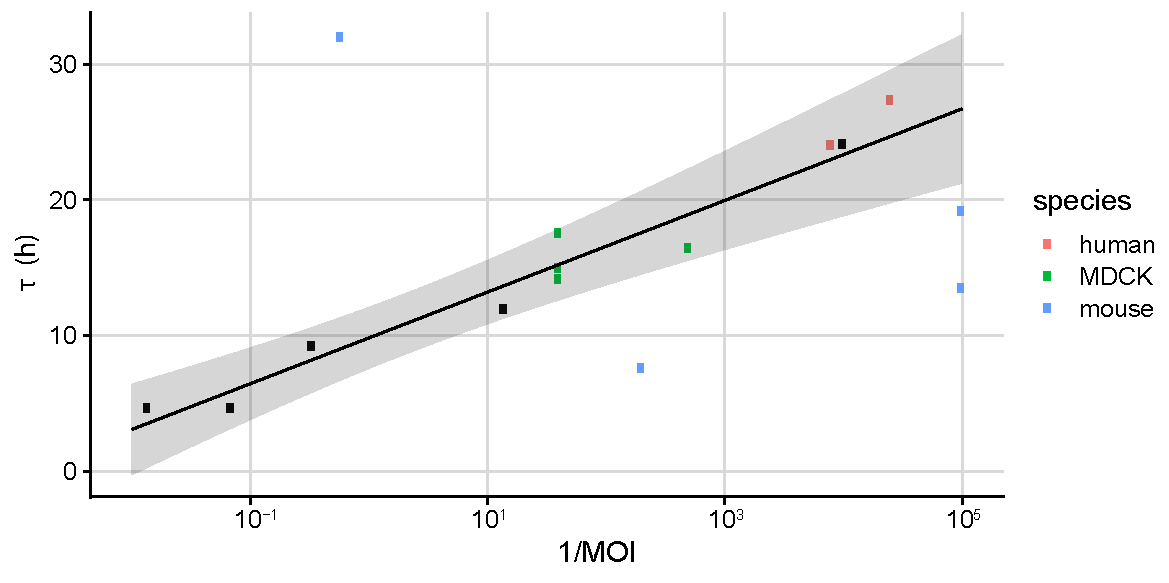
\includegraphics[width=0.95\textwidth, trim={0cm 0cm 0cm 0cm}, clip]{D_chapters/3_DARPinModels/DelayMoiValidation.pdf}
\caption[Influenza virus infection delay as a function of initial MOI]%
{Influenza virus infection delay as a function of initial MOI. \par
Black datapoints correspond to \cite{frensing2016influenza, rudiger2019multiscale, DarpinData} data used to fit the model. Red, green, and blue points correspond to the data calculated based on the delay times estimated from other publications, and the corresponding MOI.}
\label{figure:delayMoiValidation}
\end{center}
\end{figure}

To analyze the dependency between $\tau$ and MOI (Figure \ref{figure:delayMoiValidation}) we use an available literature dataset \cite{frensing2016influenza, rudiger2019multiscale} which reports influenza virus production for three values of MOI = $73$, $3$, $10^{-4}$, and WT measurements in our collaborators DARPin-F10 data \cite{DarpinData}.

Observed delay times were calculated based on an asymptotic regression function, fitted on the viral production data. Based on experimental observations, we used considerations that the dependency must have inverse proportionality to MOI, and that based on the observed delay values it is at least logarithmic. We fitted the resulting relationship between delay time $\tau$ and MOI:

\begin{equation}
\tau = a + b \log_e \Big(\frac{1}{MOI}\Big)
\label{eq:delayMOI}
\end{equation}

where $a$ = 9.83 is the delay for MOI = 1, and $b$ = 1.47 is the slope coefficient. It is worth to note that MOI = 1 has a special meaning corresponding to number of viral particles being equal to the number of target cells, making it a characteristic point for this expression.

The relationship in Equation \ref{eq:delayMOI} would break down at the very high values of MOI, both due to mathematical limitation - at $\tau$ turning negative, and biological considerations - no matter how much virus we add to the system, there will always be lag time due to internalization and uncoating processes within the cell. However, in practice, such high MOI values are used in experiments relatively rarely, and even MOI = 73 is an extreme.

Our validation using other experimental data shows that human and Madin-Darby canine kidney (MDCK) cell culture data fit our delay-MOI relationship quite well, while mice results disagree. This discrepancy may be explained by the difficulty of measuring the exact amounts of virus inhaled during the experiment by the mouse. However, in both human and mice experiments the number of observed data points is not very high, so their predictive power may vary.

\subsection{Characterising the fraction of infectious virus production}

During influenza infection viruses often produce virions which do not carry the full set of vRNPs, or are damaged in some other way. Those faulty viral particles are called defective interfering particles (DIPs). Their ability to infect and propagate relies on coinfection with fully infectious viral particles, but coinfected cells tend to release primarily progeny DIPs \cite{frensing2014impact}. At high MOI values most cells are infected with several virions, providing the best conditions for DIP accumulation. Thus, another quantity of interest is infectious fraction - the fraction of infectious viral particles compared to total viral particles produced during the infection:

\begin{equation}
    \text{Infectious fraction} = \frac{\text{Infectious viral particles}}{\text{Total viral particles}}
\end{equation}

\begin{figure}
\begin{center}
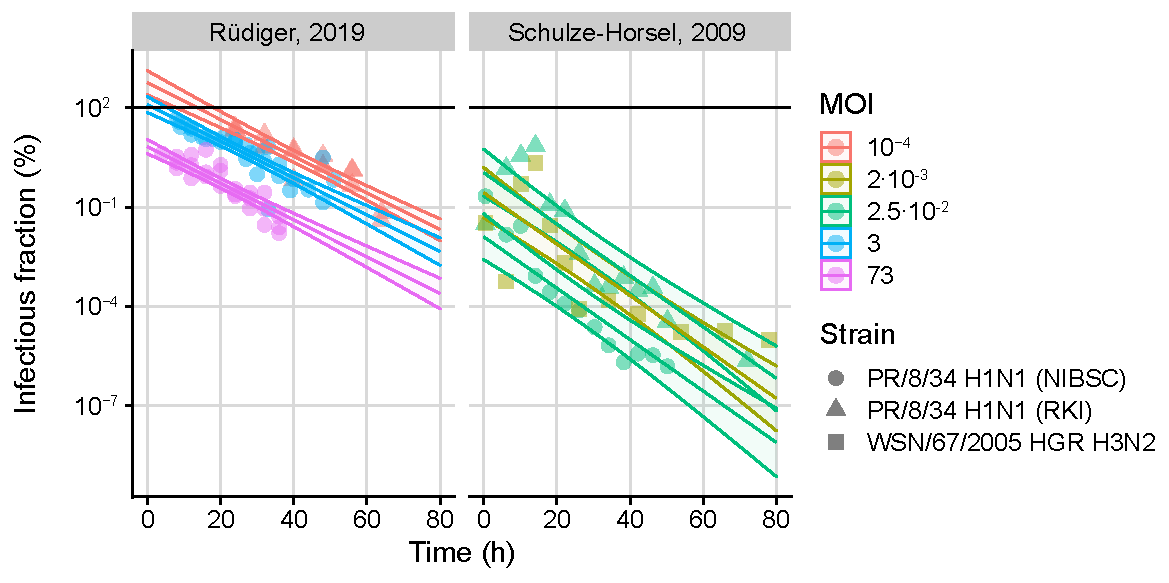
\includegraphics[width=0.95\textwidth, trim={0cm 0cm 0cm 0cm}, clip]{D_chapters/3_DARPinModels/InfectiousFractionAll.pdf}
\caption[Infectious fraction of virus production over the course of infection]%
{Infectious fraction of virus production over the course of infection for 3 different strains and 5 values of MOI, based on the data from \cite{frensing2016influenza, rudiger2019multiscale} and digitalized data from \cite{schulze2009infection}. Each panel has been fitted as a parallel slope model, R\"udiger, 2019 \cite{rudiger2019multiscale} based on MOI, and Schulze-Horsel, 2009 \cite{schulze2009infection} based on the strain used.}
\label{figure:infectiousFraction}
\end{center}
\end{figure}

A simple plot of infectious fraction \cite{rudiger2019multiscale, frensing2016influenza} as a function of time after infection reveals a linear relationship between the two, offset by the MOI value (Figure \ref{figure:infectiousFraction}, left). Unfortunately, with just 3 data points we can only observe that in accordance with our expectations high MOI leads to a low infectious fraction, but this relationship may be confounded by the use of two different viral strains.

Another study \cite{schulze2009infection} uses the same two strains, along with one H3N2 strain, at two different values of MOI, so we used their digitized data to plot the infectious fraction, hoping for an additional insight. Regardless of specific strain and MOI used, infectious fraction still displays a similar log-linear relationship with time. However, it is apparent that the overall infectious fraction is lower than what was observed in \cite{rudiger2019multiscale, frensing2016influenza} by about 3 orders of magnitude, despite the fact that the MOI values used by \cite{schulze2009infection} are relatively low. Whether that is due to their use of microcarrier culture, or simply an artifact of preparation is unclear.

Unfortunately, these discrepancies in experimental data do not allow us to make quantitative predictions about the relationship between infectious fraction, MOI, and viral strains, but they present an interesting case for future research efforts.

\subsection{Influenza infection model selection}

Literature dataset \cite{rudiger2019multiscale} displayed a slow depletion of target cells over the course of infection, prompting us to consider chronic models and models with a target cell population described by a fitted Hill equation. For chronic models the target cell population is slowly renewed over the course of infection with a constant rate $g$. For models with a target cell population described by a fitted Hill equation, the infection is limited by target cell availability later in the infection:

\begin{equation}
T = \frac{T_0}{1+\exp \big(n^{Target}\log_e(\frac{EC_{50}^{Target}}{T})\big)}
\end{equation}

where $T$ is the current number of target cells, $T_0$ is the initial number of target cells, $EC_{50}^{Target}$ is a half maximal effective concentration of target cells, $n^{Target}$ is a Hill coefficient of target depletion.

To model influenza virus infection, we prepared two chronic and seven depletion infection models, which we named after the states and parameters they include (Figure \ref{figure:compartamentalSchematic}, Appendix \ref{appendix:compartmentalModelEquations}). We fitted these models (Table \ref{table:ModelObjFunction}) using literature data \cite{rudiger2019multiscale, frensing2016influenza} for three values of MOI. Judging by the objective function values, as well as visual evaluation of the fits (Appendix \ref{appendix:compartmentalModelFits}), models with a target cell population described by a fitted Hill equation performed the best, reaching objective function values about an order of magnitude lower than the next candidates (Table \ref{table:ModelObjFunction}). In the following analysis we only focus on these three models.

\begin{figure}
\begin{center}
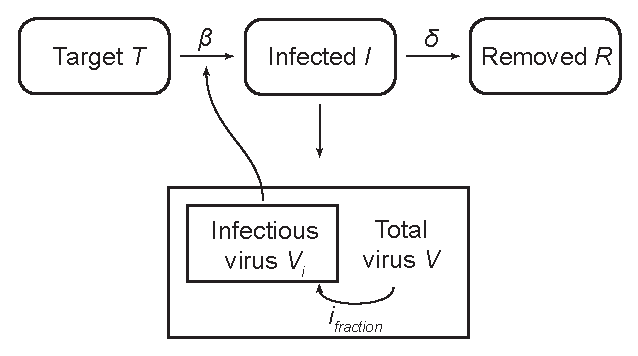
\includegraphics[width=0.95\textwidth, trim={0cm 0cm 0cm 0cm}, clip]{D_chapters/3_DARPinModels/compartamentalSchematic.pdf}
\caption[Schematic representation of a simple TIRVV$_i$ kinetic model]{Schematic representation of a simple TIRVV$_i$ kinetic model \par
Rectangles represent virus populations, and rounded rectangles represent cell populations. Arrows indicate transitions between populations.}
\label{figure:compartamentalSchematic}
\end{center}
\end{figure}

\newpage

\begin{figure}[H]
\begin{center}
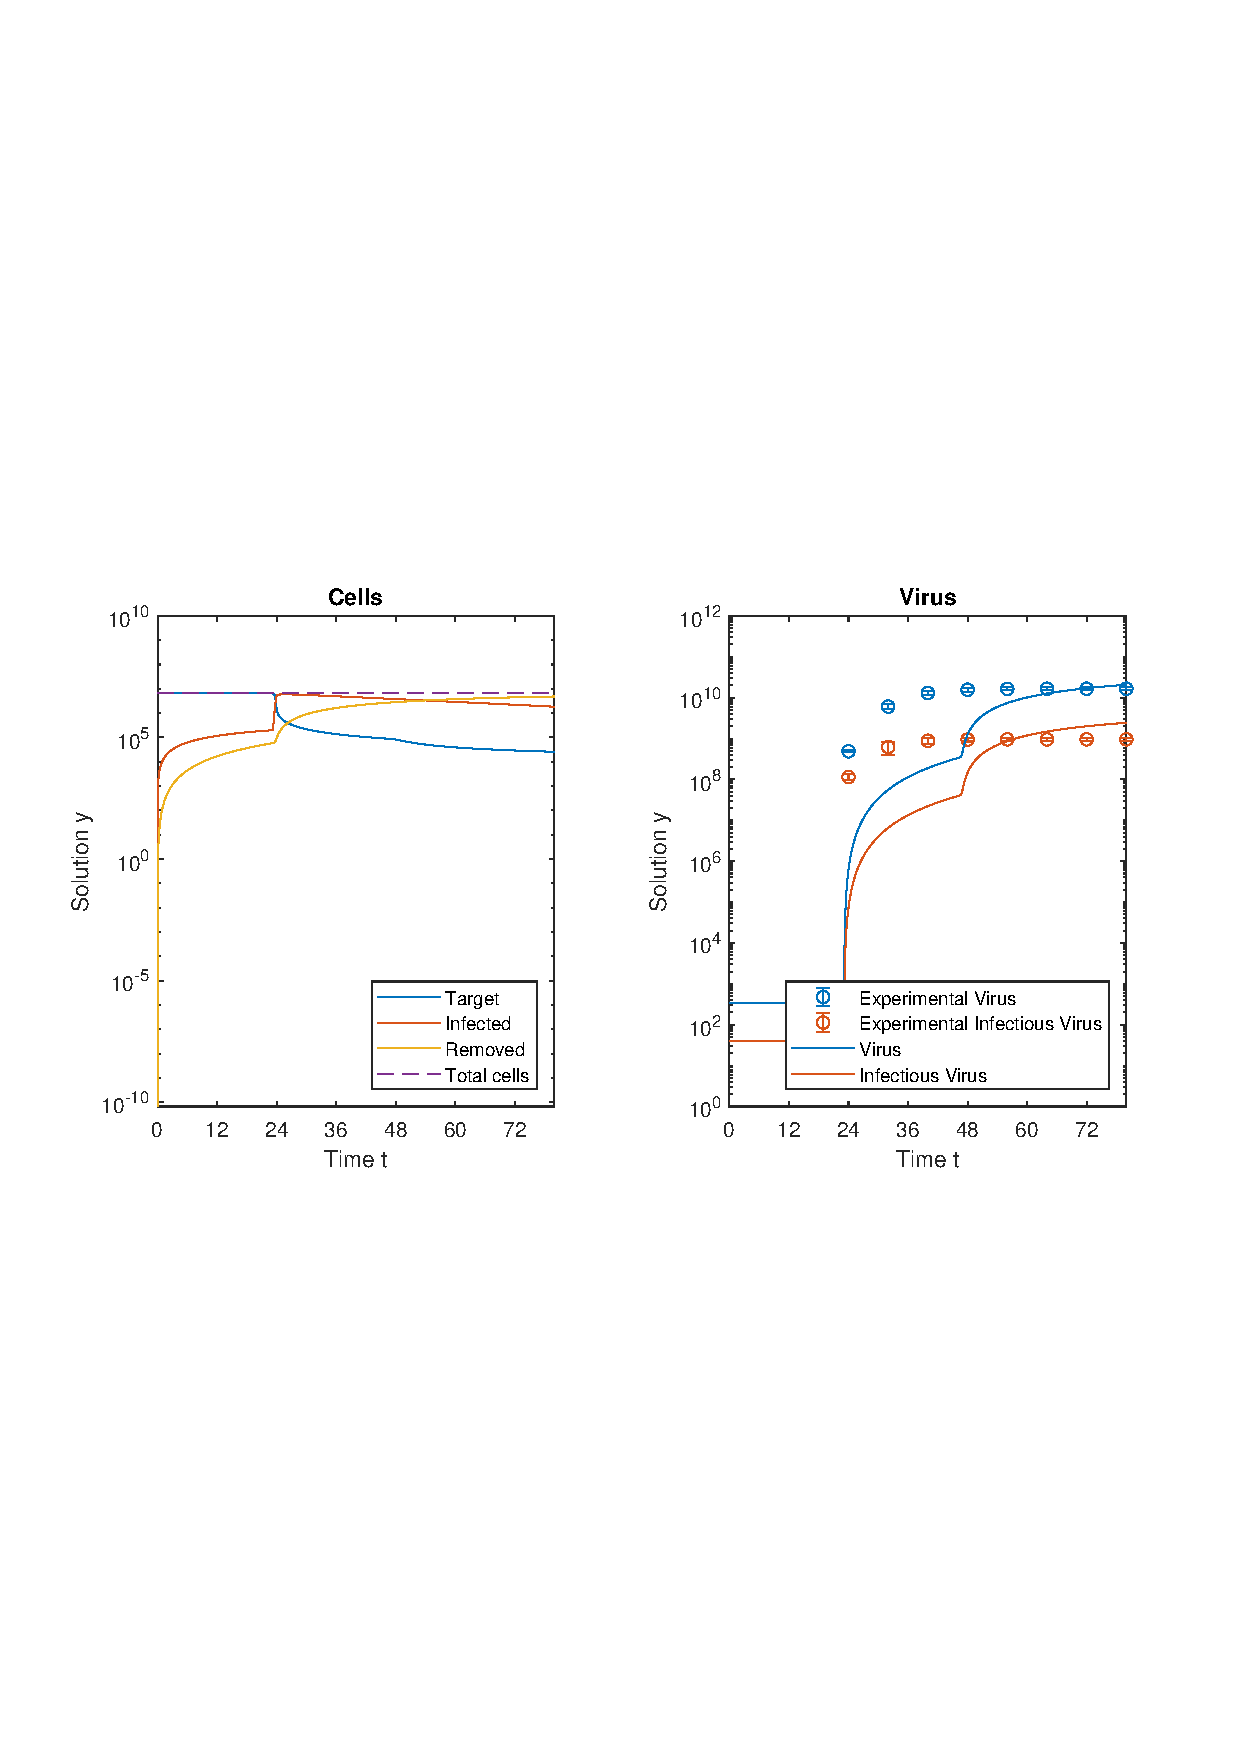
\includegraphics[width=0.6\textwidth, trim={1cm 9.5cm 1cm 9.5cm}, clip]{D_chapters/6_appendix/4_THillIRVViDelay/ModelTHillIRVViDelayDSNSaenz2010FittedMOI0.0001B0.0010133D0.55548P3247.2256C0.0027335TIC1896440.1965TH4.9813iFrac0.11736log.pdf}
\caption[T$_{Hill}$IRVV$_i$, delay $\tau = f(\text{MOI})$ model fit for MOI = $10^{-4}$]%
{T$_{Hill}$IRVV$_i$, delay $\tau = f(\text{MOI})$ model fit for MOI = $10^{-4}$}
\label{figure:THillIRVViDelayMOI00001}
\end{center}
\end{figure}

\begin{figure}[H]
\begin{center}
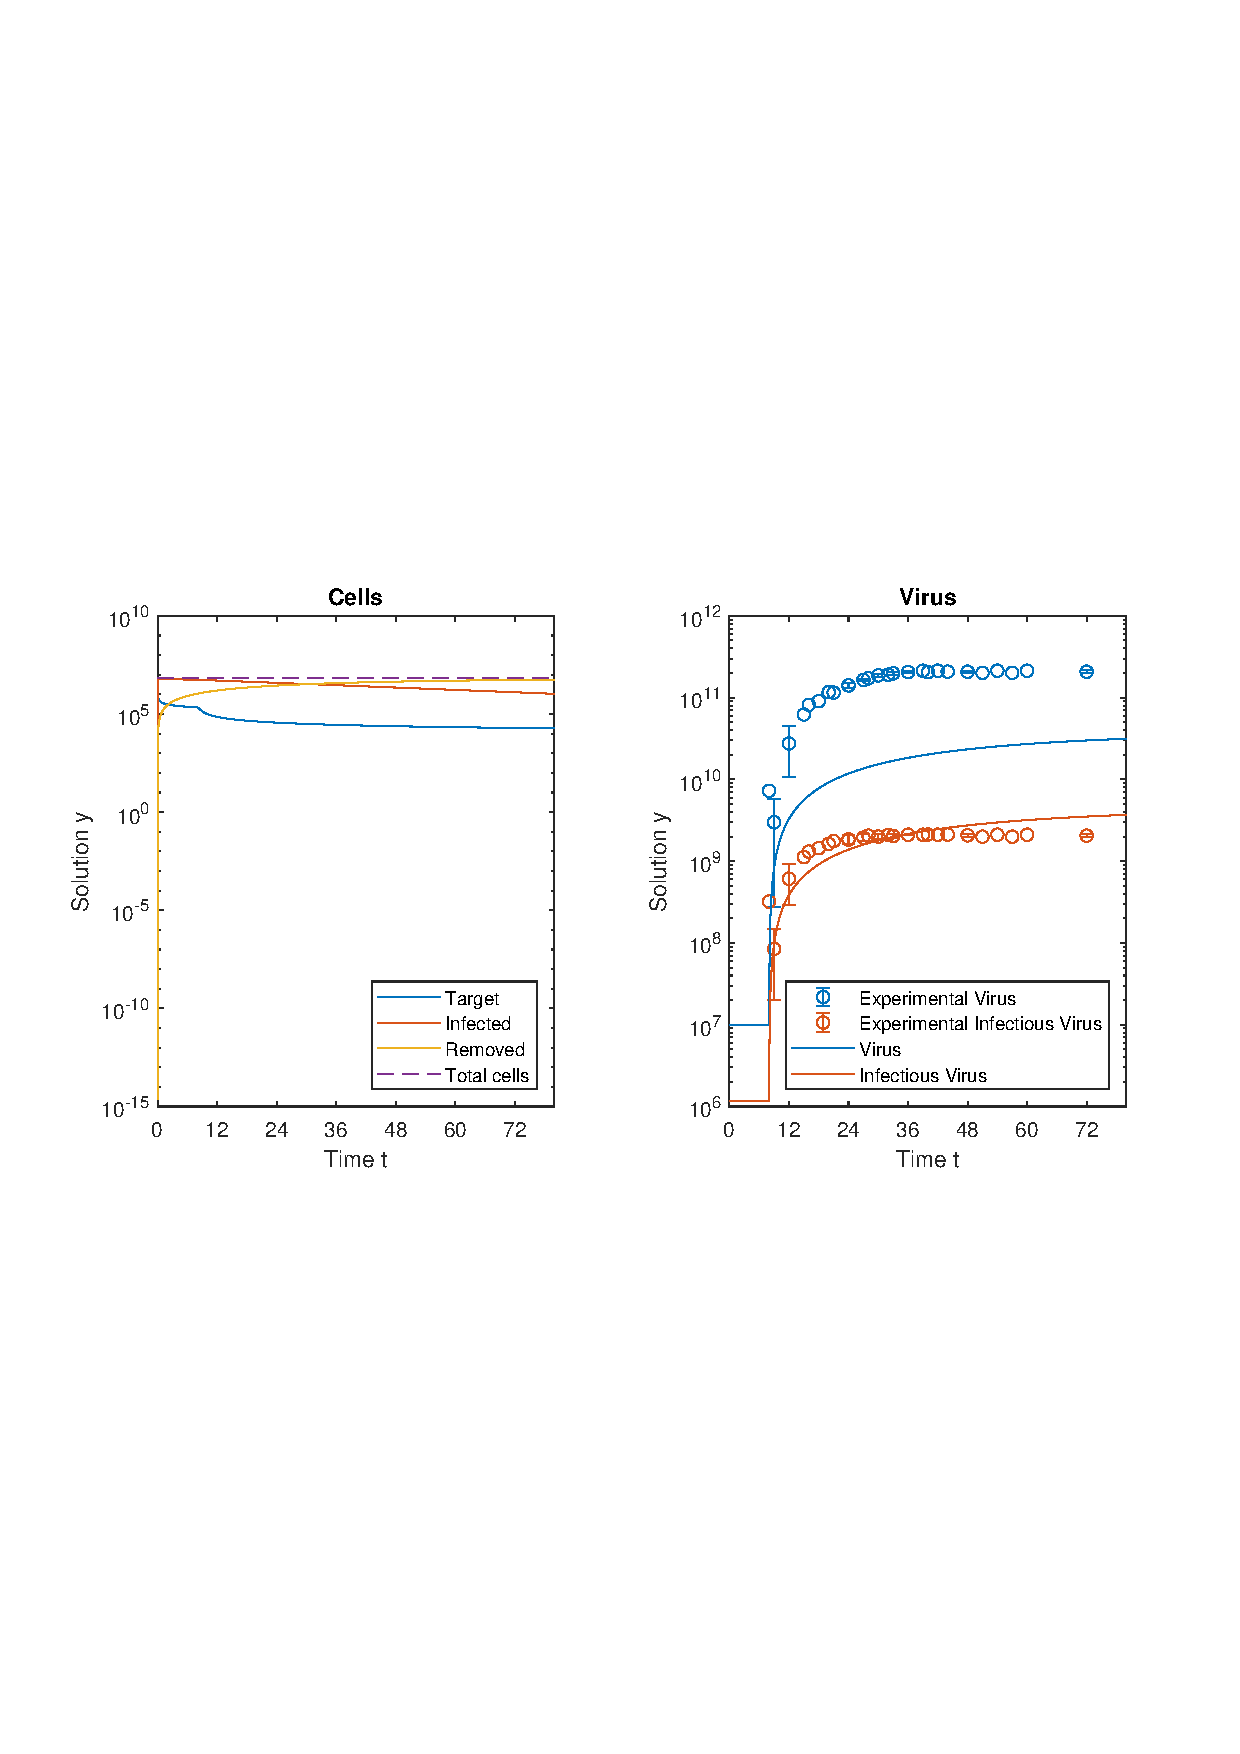
\includegraphics[width=0.6\textwidth, trim={1cm 9.5cm 1cm 9.5cm}, clip]{D_chapters/6_appendix/4_THillIRVViDelay/ModelTHillIRVViDelayDSNSaenz2010FittedMOI3B0.0010133D0.55548P3247.2256C0.0027335TIC1896440.1965TH4.9813iFrac0.11736log.pdf}
\caption[T$_{Hill}$IRVV$_i$, delay $\tau = f(\text{MOI})$ model fit for MOI = 3]%
{T$_{Hill}$IRVV$_i$, delay $\tau = f(\text{MOI})$ model fit for MOI = 3}
\label{figure:THillIRVViDelayMOI3}
\end{center}
\end{figure}

\begin{figure}[H]
\begin{center}
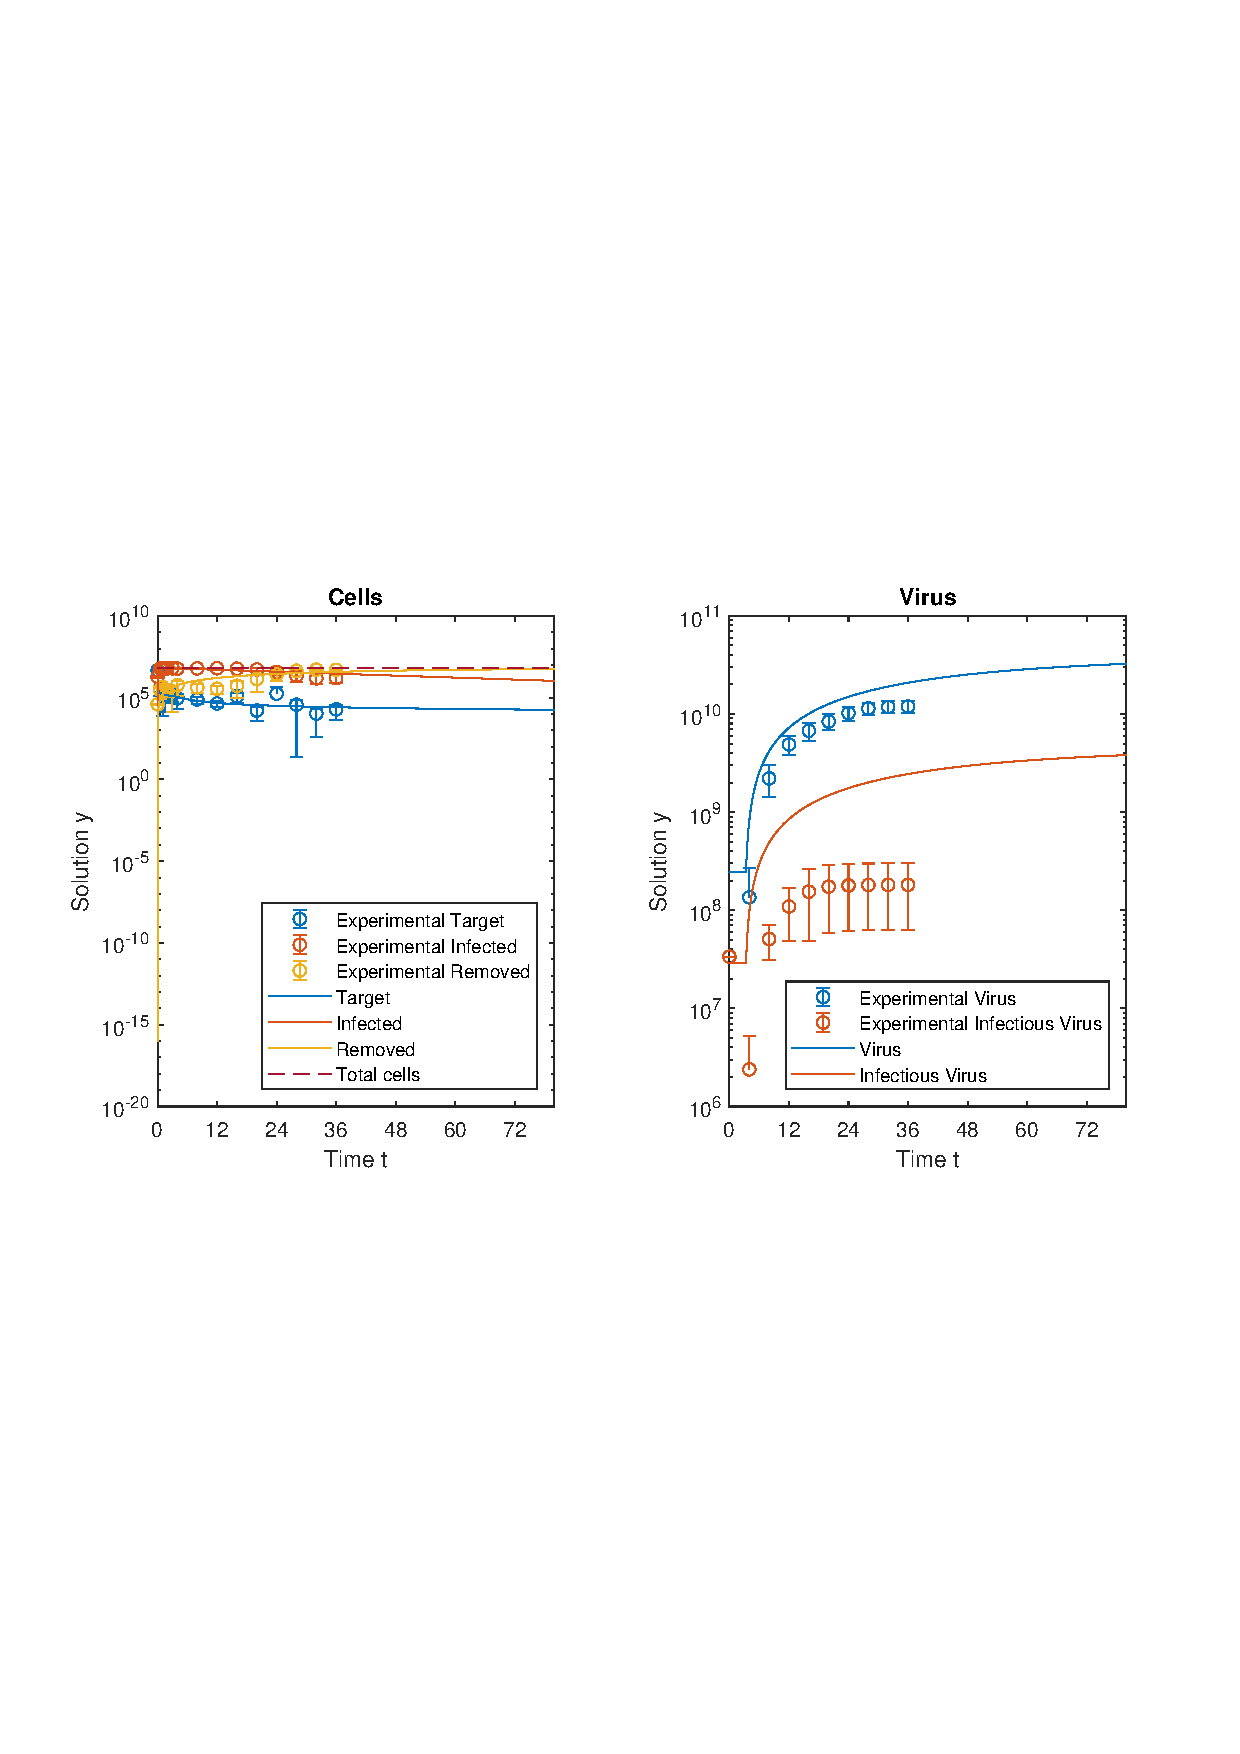
\includegraphics[width=0.6\textwidth, trim={1cm 9.5cm 1cm 9.5cm}, clip]{D_chapters/6_appendix/4_THillIRVViDelay/ModelTHillIRVViDelayDSNSaenz2010FittedMOI73B0.0010133D0.55548P3247.2256C0.0027335TIC1896440.1965TH4.9813iFrac0.11736log.pdf}
\caption[T$_{Hill}$IRVV$_i$, delay $\tau = f(\text{MOI})$ model fit for MOI = 73]%
{T$_{Hill}$IRVV$_i$, delay $\tau = f(\text{MOI})$ model fit for MOI = 73}
\label{figure:THillIRVViDelayMOI73}
\end{center}
\end{figure}

Despite the objective function scores, visual evaluation of the fits (Figures \ref{figure:THillIRVViDelayMOI00001}, \ref{figure:THillIRVViDelayMOI3}, \ref{figure:THillIRVViDelayMOI73}, Appendix \ref{appendix:compartmentalModelFits}, only models which describe target cell population by a fitted Hill equation fits reported) reveals that T$_{Hill}$IRVV$_i$ does not capture the initial delay in the viral production, and all three models struggle to capture the infectious fraction, which in all models is set to be constant (which we know is not the case, as shown on Figure \ref{figure:infectiousFraction}). T$_{Hill}$IRVV$_i$, delay $\tau = f(\text{MOI})$ model predicts an extra viral production bump for low MOI = $10^{-4}$. T$_{Hill}$IRVV$_i$, delay $\tau = const$ suggests one as well, but early in the infection, before the literature reported data points.

\begin{table}[h!]
\centering
\caption[Influenza infection model objective function values for best fits]{Influenza infection model objective function values for best fits}
\label{table:ModelObjFunction}

\begin{tabular}{p{8cm} p{3cm} p{2.5cm}}
\hline 
\textbf{Infection model} & \textbf{Objective function value} & \textbf{Fitted \mbox{parameters}}\\
\hline
chronic TIRVV$_i$ & 2.95 & 6\\
chronic TEIRVV$_i$ & 2.30 & 7\\
\hline
TIRVV$_i$ & 2.96 & 5\\
TEIRVV$_i$ &  3.73 & 6\\
TIRVV$_i$, delay $\tau = f(\text{MOI})$ & 12.82 & 5\\
TIRVV$_i$, delay $\tau = const$ & 6.63 & 6\\
T$_{Hill}$IRVV$_i$ & 0.36 & 7\\
T$_{Hill}$IRVV$_i$, delay $\tau = f(\text{MOI})$ & 0.63 & 7\\
T$_{Hill}$IRVV$_i$, delay $\tau = const$ & 0.25 & 8\\
\hline
\end{tabular}
\end{table}

\newpage

\begin{figure}[H]
\begin{center}
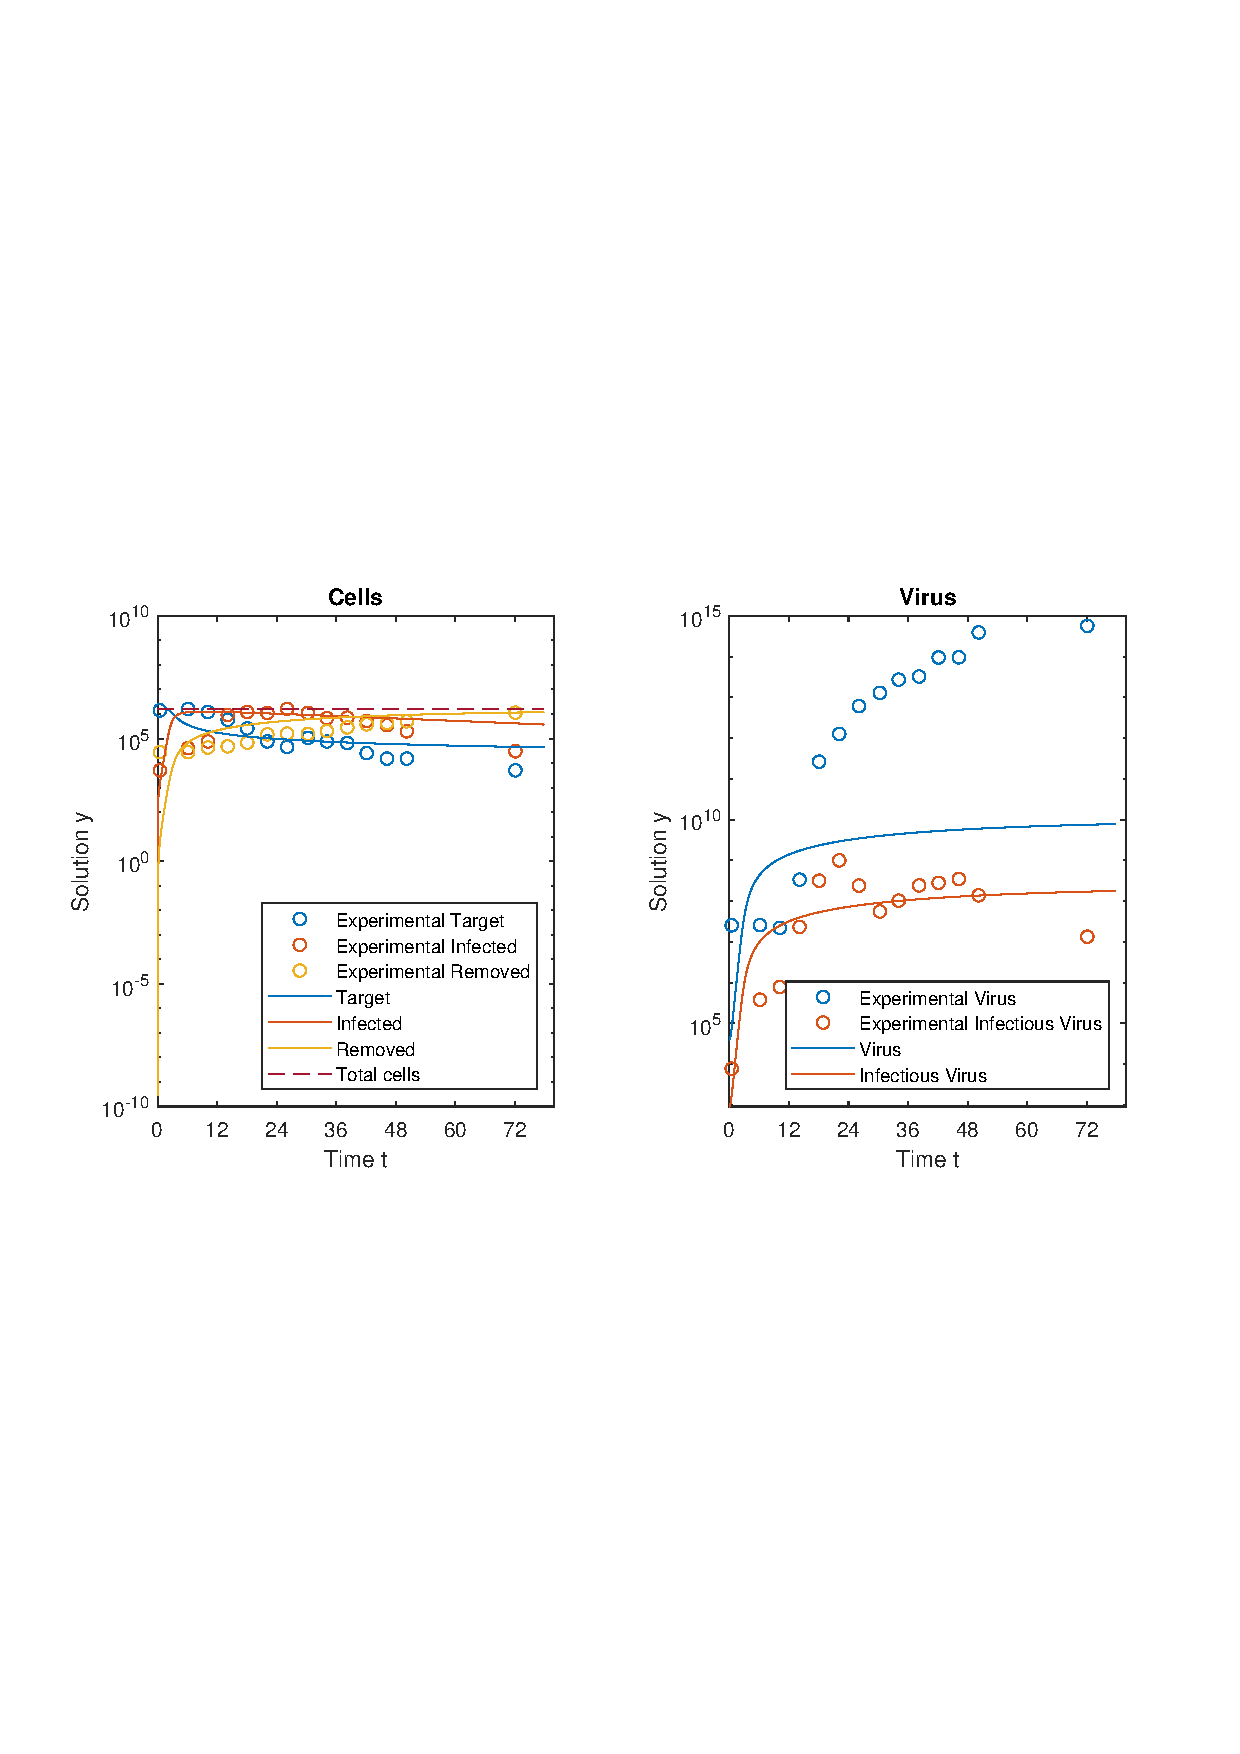
\includegraphics[width=0.65\textwidth, trim={1cm 9.8cm 1cm 9.5cm}, clip]{D_chapters/6_appendix/4_ValidationRKI/InfectionDepletionModelTHillIRVViMOI0.025log.pdf}
\caption[T$_{Hill}$IRVV$_i$ model fit for PR/8/34 H1N1 (RKI)]%
{T$_{Hill}$IRVV$_i$ model fit PR/8/34 H1N1 (RKI)}
\label{figure:THillIRVViValidationRKI}
\end{center}
\end{figure}

\begin{figure}[H]
\begin{center}
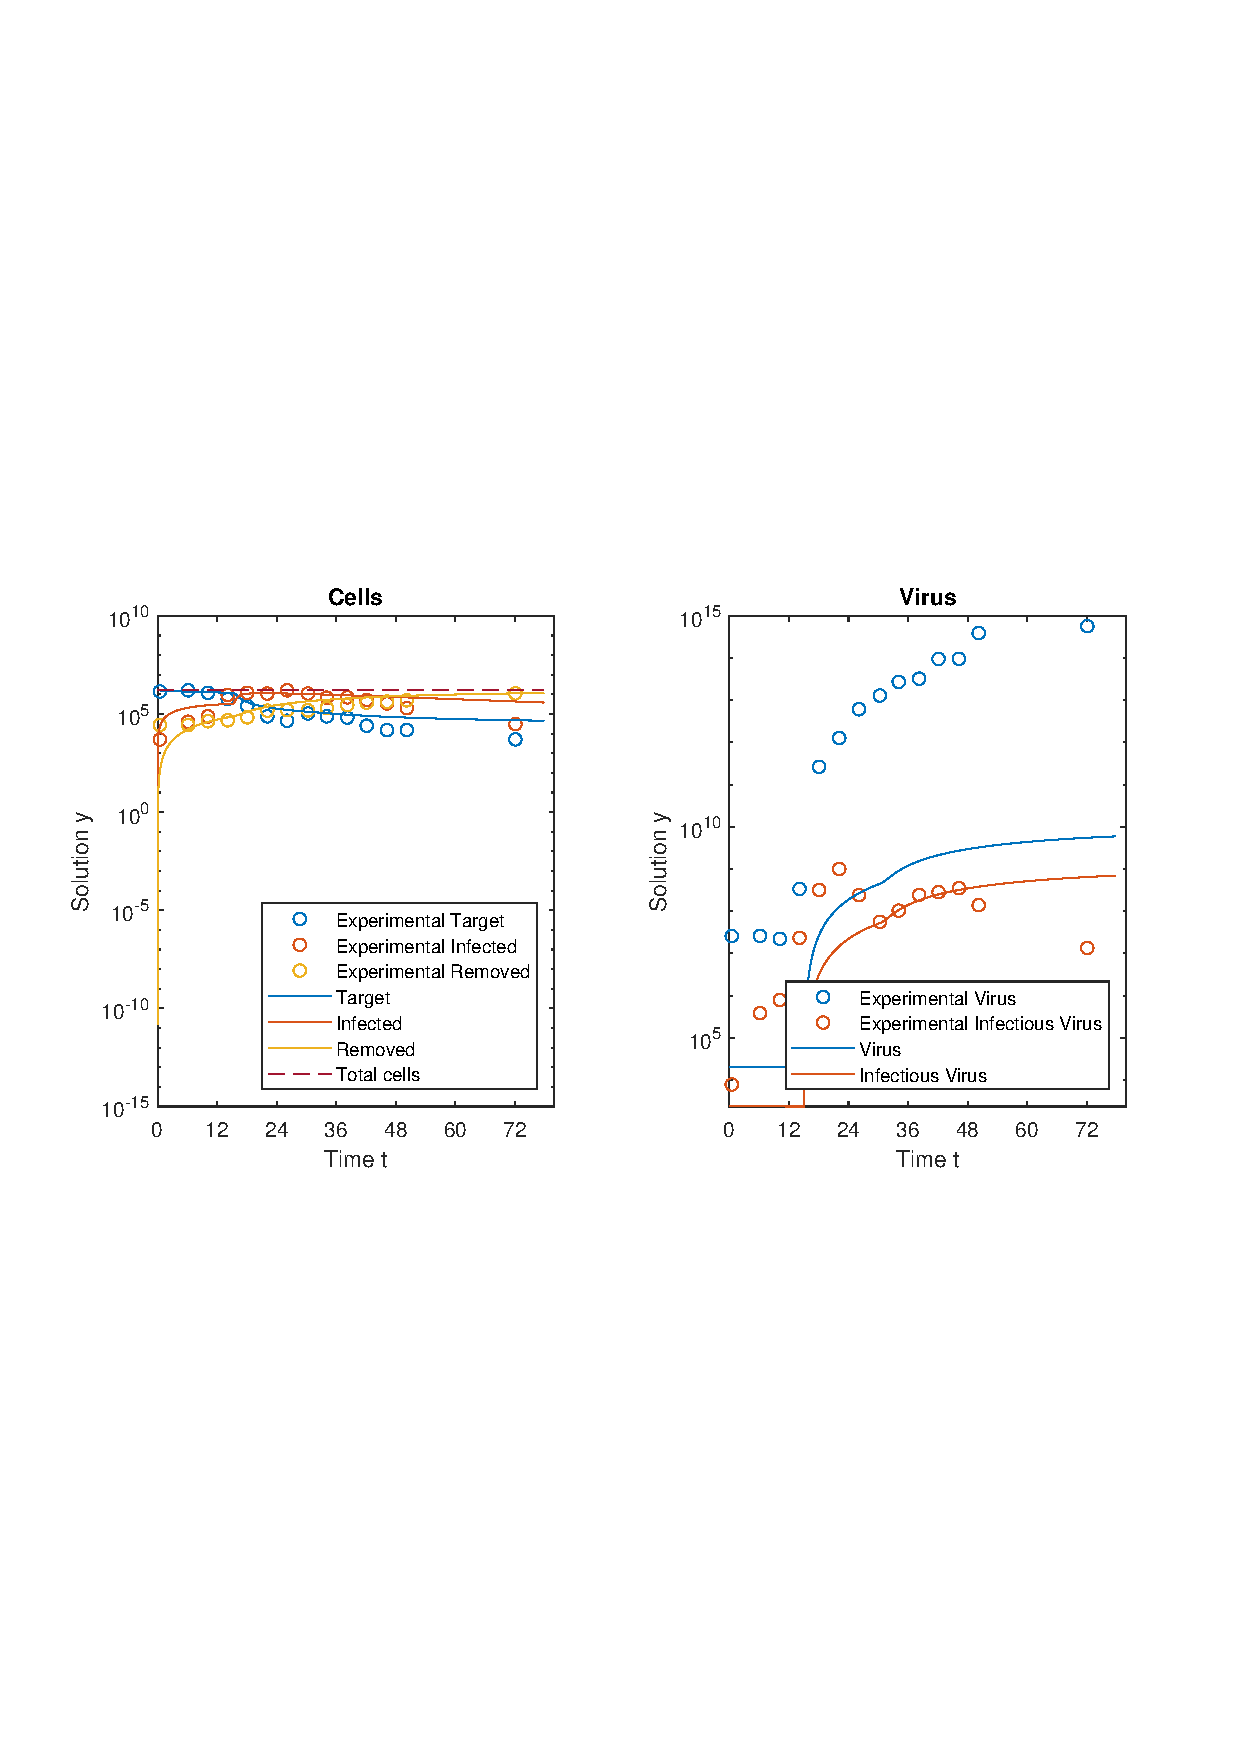
\includegraphics[width=0.65\textwidth, trim={1cm 9.8cm 1cm 9.5cm}, clip]{D_chapters/6_appendix/4_ValidationRKI/InfectionDepletionModelTHillIRVViDelayMOI0.025log.pdf}
\caption[T$_{Hill}$IRVV$_i$, delay $\tau = f(\text{MOI})$ model fit forPR/8/34 H1N1 (RKI)]%
{T$_{Hill}$IRVV$_i$, delay $\tau = f(\text{MOI})$ model fit for PR/8/34 H1N1 (RKI)}
\label{figure:THillIRVViDelayValidationRKI}
\end{center}
\end{figure}

\begin{figure}[H]
\begin{center}
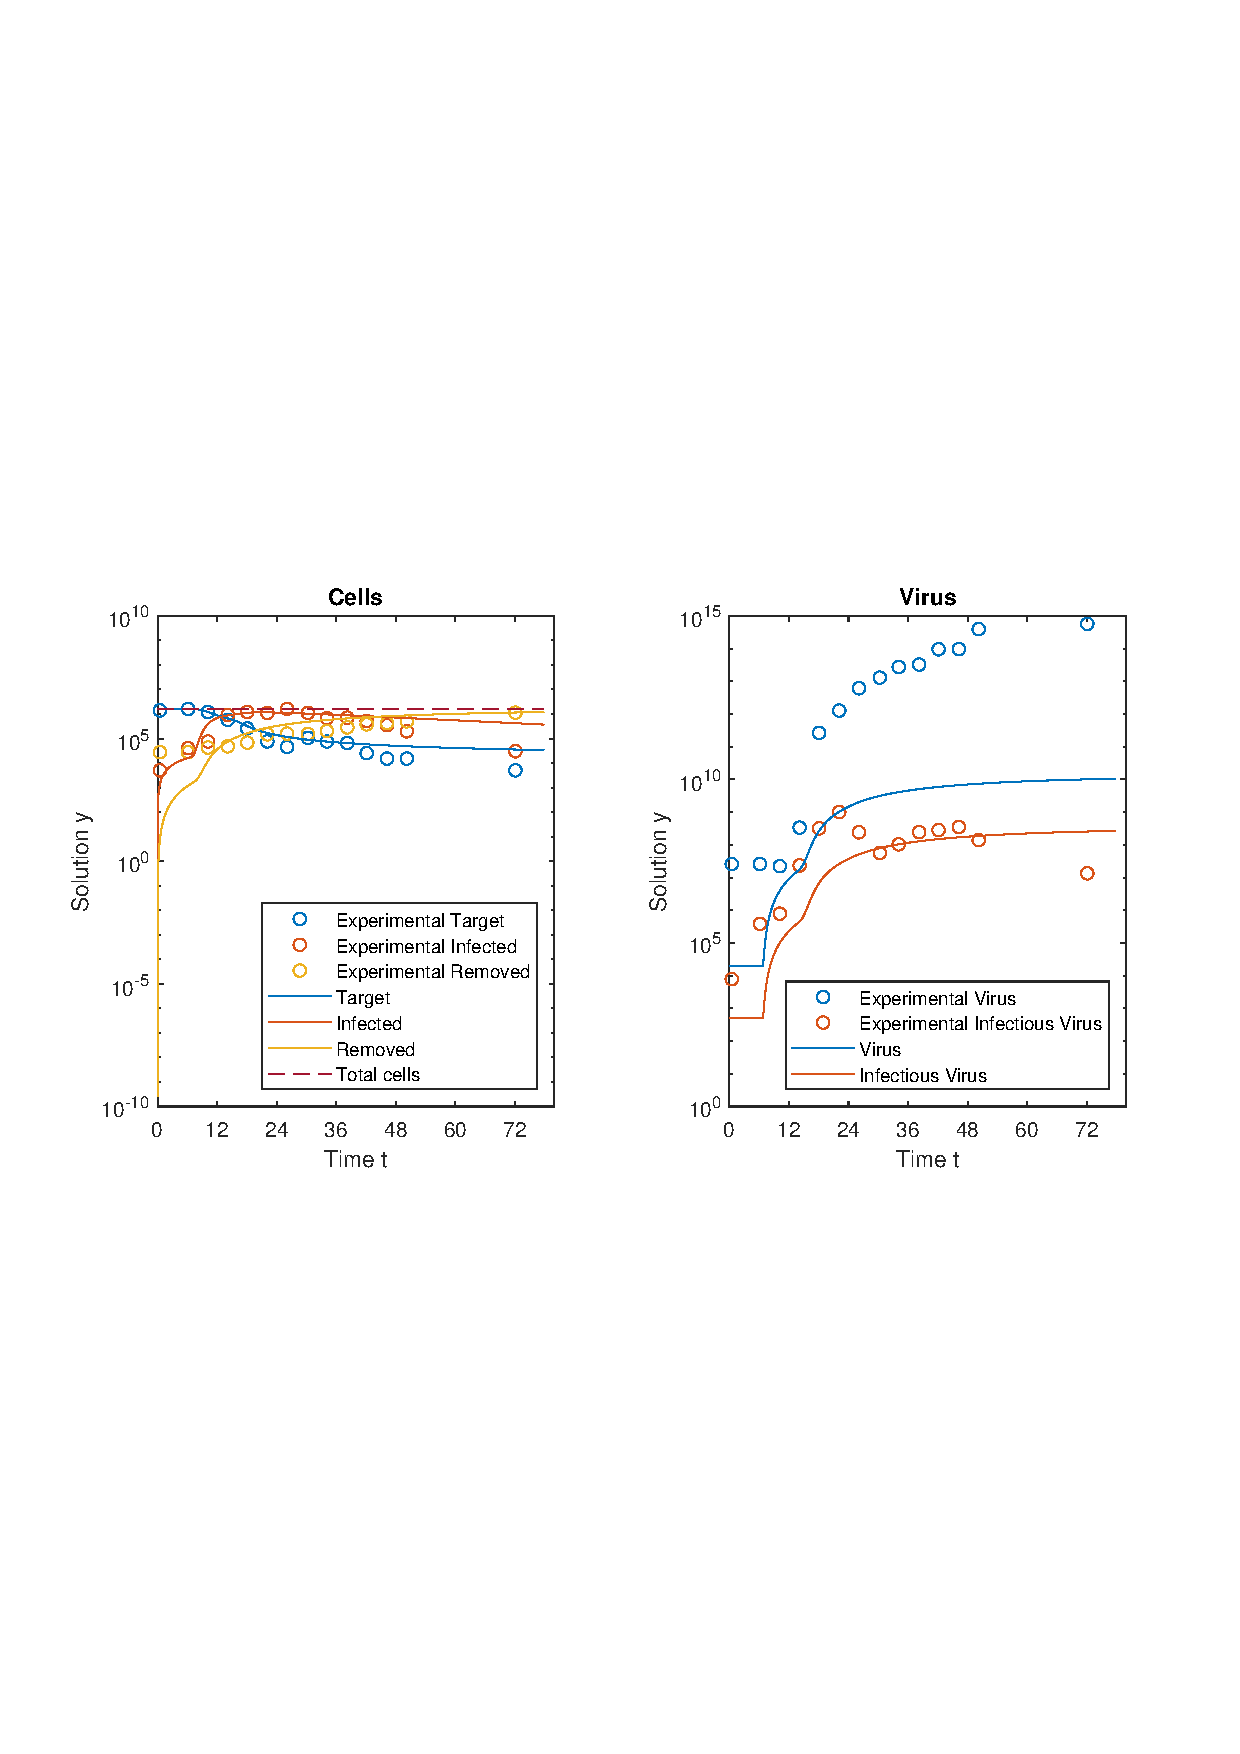
\includegraphics[width=0.65\textwidth, trim={1cm 9.8cm 1cm 9.5cm}, clip]{D_chapters/6_appendix/4_ValidationRKI/InfectionDepletionModelTHillIRVViDelayFitTauMOI0.025log.pdf}
\caption[T$_{Hill}$IRVV$_i$, delay $\tau = const$ model fit for PR/8/34 H1N1 (RKI)]%
{T$_{Hill}$IRVV$_i$, delay $\tau = const$ model fit for PR/8/34 H1N1 (RKI)}
\label{figure:THillIRVViDelayFitTauValidationRKI}
\end{center}
\end{figure}

To evaluate the practical usability of these fits, we used them to run the simulations with initial conditions corresponding to the ones reported in \cite{schulze2009infection}, and visually compared the resulting trajectories with digitized data from \cite{schulze2009infection}. For all the viral strains our best fit candidates again performed the best (Figures \ref{figure:THillIRVViValidationRKI}, \ref{figure:THillIRVViDelayValidationRKI}, \ref{figure:THillIRVViDelayFitTauValidationRKI}, Appendix \ref{appendix:compartmentalModelFitValidation}). However, all three models struggled significantly to capture the infectious fraction. As previously discussed, this discrepancy may be explained by the infectious fraction in \cite{schulze2009infection} being significantly reduced compared to our fitting data \cite{rudiger2019multiscale}. Interestingly, for PR/8/34H1N1 (RKI) and WSN/67/2005 HGR H3N2 strains the infectious virions trajectory was simulated reasonably well by the models, unlike for PR/8/34H1N1 (NIBSC), which had the worst infectious fraction out of all the strains reported in \cite{schulze2009infection}.

Out of all the simulated models T$_{Hill}$IRVV$_i$, delay $\tau = const$ and T$_{Hill}$IRVV$_i$, delay $\tau = f(\text{MOI})$ seem to perform the best, in terms of capturing both cellular behavior and overall shape of the viral production. Unfortunately, we cannot say that modelling delay $\tau = f(\text{MOI})$ as a function of MOI offers any significant advantage over $\tau = const$, but it is worth noting that $\tau = const$ requires fitting $\tau$ as an additional parameter of the infection model, where $\tau = f(\text{MOI})$ relies on a pre-computed expression.

\subsection{DARPin-F10 drug-like activity}

To model the drug-like activity of DARPin-F10, we modified our fitted infection models T$_{Hill}$IRVV$_i$, delay $\tau = const$ and T$_{Hill}$IRVV$_i$, delay $\tau = f(\text{MOI})$ to include DARPin-F10. Ultimately, both model variants have produced qualitatively similar results, so here we only present the simulation results for T$_{Hill}$IRVV$_i$, delay $\tau = f(\text{MOI})$.

We examined two possible cases: one where DARPin-F10 behaves similarly to amantadine drug, reducing the infection rate $\beta$, and another, where it behaves similarly to neuraminidase inhibitors, reducing the virion production $p$.

To model DARPin-F10 influence on the infection we used parametrised dose response curves (Table \ref{table:DARPinFittingCoefficients}) obtained from modified HDAC6 complex formation models "Asymmetric DARPin" and "Symmetric DARPin" to compute the drug effect, under assumption that the DARPin-F10 concentration stays constant throughout simulation. Since in the limit where DARPin-F10 = 0 our predictions for dose response would be the same as the WT conditions, for simplicity we assumed that $\epsilon_{max} - \epsilon_{min} = 1$. Both "Asymmetric DARPin" and "Symmetric DARPin"  sets of parameters produced qualitatively similar results, so here we only present the results for "Asymmetric DARPin".

Surprisingly, an amantadine-like model (Figure \ref{figure:amantadineLikeF210}, Appendix \ref{appendix:amantadineDarpin}) only led to a moderate decrease in viral production. In this model DARPin-F10 reduces infection rate $\beta$, leading to slower target cell depletion (Figure \ref{figure:amantadineLikeF210}, orange line), to a slower increase in the number of infected cells (Figure \ref{figure:amantadineLikeF210}, yellow line), and to less steep virus production (Figure \ref{figure:amantadineLikeF210}, blue line). This model captures the overall smoother shape of the DARPin-F10 inhibited viral growth at the start of the infection (Figure \ref{figure:amantadineLikeF210}, $\le 36$ hours), but the simulated virus production does not quite reach experimentally observed reduction even at high concentration of DARPin-F10 (Figure \ref{figure:amantadineLikeF210} $[F]_{effective}$ = 210.24 = 7.3 $\mu$M.

\begin{figure}
\begin{center}
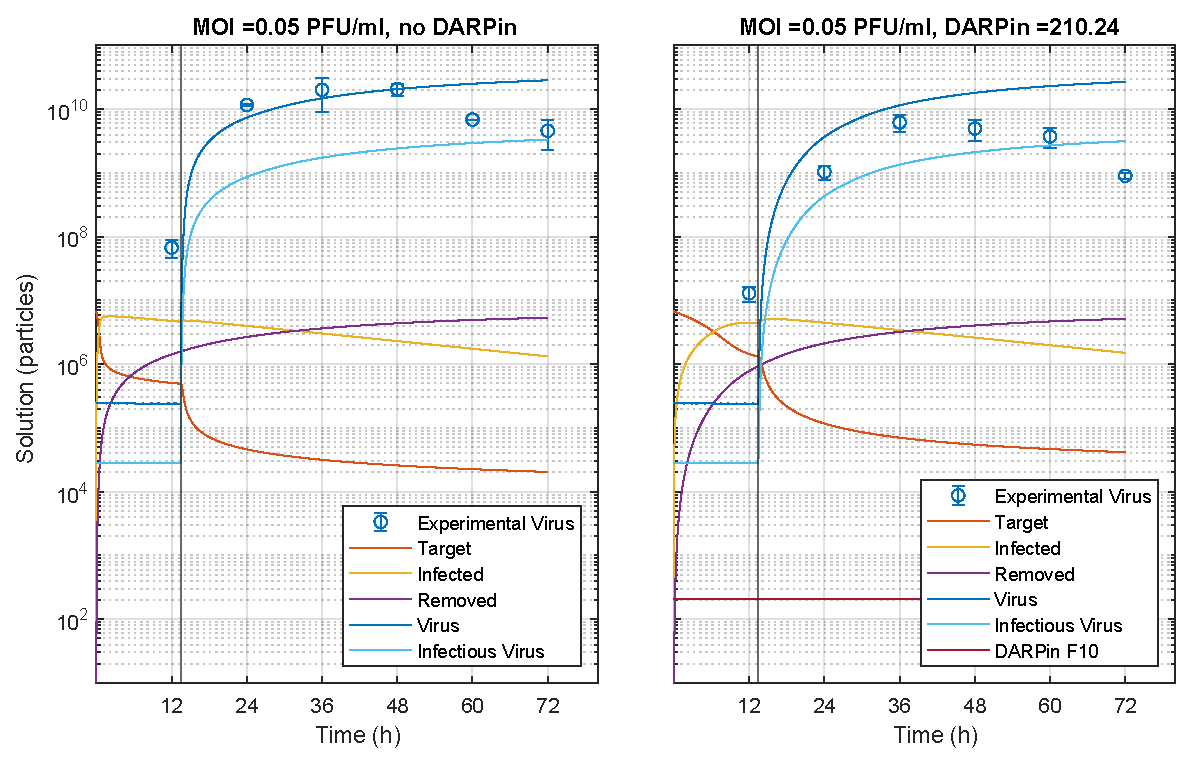
\includegraphics[width=0.8\textwidth, trim={0cm 0cm 0cm 0cm}, clip]{D_chapters/3_DARPinModels/2_DARPinInfection/comparisonModelTHillIRVViDelayMOI0.072135DARPin210.236AsymmetricDarpinMyosinInhibitor.pdf}
\caption[Amantadine-like DARPin-F10 for MOI = 0.05 PFU/ml and $F_{effective}$ = 210.24]{Amantadine-like DARPin-F10 influence on the influenza infection for MOI = 0.05 PFU/ml and relative DARPin-F10 $[F]_{effective}$ = 210.24, calculated based on viral growth curves at MOI = 10 PFU/ml. Experimental data is normalized to  the simulated virus production value at 48h for no DARPin case.}
\label{figure:amantadineLikeF210}
\end{center}
\end{figure}

Neuraminidase inhibitor-like models (Figures \ref{figure:neuraminidaseInhibitorLikeF62}, Appendix \ref{appendix:neuraminidaseInhibitorDarpin}) were able to capture the reduction in viral production far more successfully, particularly for $[F]_{effective}$ = 62.69 = 2.2 $\mu$M, determined from viral growth curves at MOI = 0.05 PFU/ml (Figure \ref{figure:neuraminidaseInhibitorLikeF62}). In this model DARPin-F10 reduces production rate $p$, directly decreasing the numbers of total (Figure \ref{figure:neuraminidaseInhibitorLikeF62}, blue line) and infectious (Figure \ref{figure:neuraminidaseInhibitorLikeF62}, light blue line) virus in the system. This may indicate that inhibition of HDAC6-Ub binding during HDAC6-mediated uncoating leads to disruption of HDAC6-assisted viral particle assembly.

\begin{figure}
\begin{center}
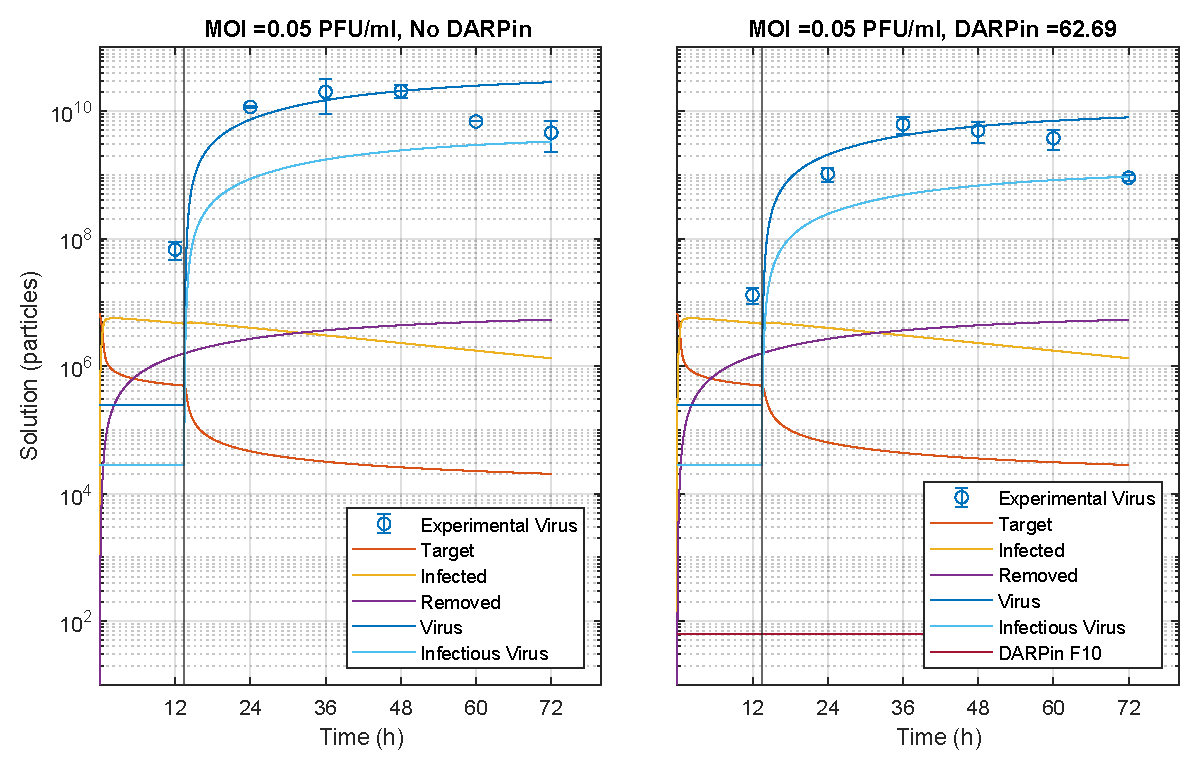
\includegraphics[width=0.8\textwidth, trim={0cm 0cm 0cm 0cm}, clip]{D_chapters/3_DARPinModels/2_DARPinProduction/comparisonModelTHillIRVViDelayMOI0.072135DARPin62.6898AsymmetricDarpinMyosinInhibitor.pdf}
\caption[Neuraminidase inhibitor-like DARPin-F10 for MOI = 0.05 PFU/ml and $F_{effective}$ = 62.69]{Neuraminidase inhibitor-like DARPin-F10 influence on the influenza infection for MOI = 0.05 PFU/ml and relative DARPin-F10 $[F]_{effective}$ = 62.69, calculated based on viral growth curves at MOI = 0.05 PFU/ml. Experimental data is normalized to the simulated virus production value at 48h for no DARPin case.}
\label{figure:neuraminidaseInhibitorLikeF62}
\end{center}
\end{figure}